\section{Flipping Edges}
\label{sect:flipping-edges}

Let us now discuss the aforementioned edge flip. An internal edge $\{u,v\}$ is incident to two different internal faces $f$, $g$. Let $x$ and $y$ denote the third vertex bounding $f$ and $g$, respectively. It is $x \neq y$ because the cluster graph is simple. Flipping the edge $\{u,v\}$ would replace it with the edge $\{x,y\}$. This operation is therefore only permitted if $x$ and $y$ are not already adjacent \emdash{} otherwise we would introduce a duplicate adjacency. A valid edge flip operation is illustrated in \cref{fig:flip-internal-edge-example}.

%let p1 denote first bend on boundary after p3
%include yellow face in 4.10? make alternating clearer. make angle thing clearer and what happens if more than 180. why do we repeat on other side?

\begin{figure}[H]
	\centering
	\subfigure[]{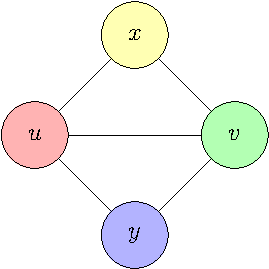
\includegraphics[height=29mm]{Resources/FlipInternalEdge-Example-1.pdf}}
	\quad
	\subfigure[]{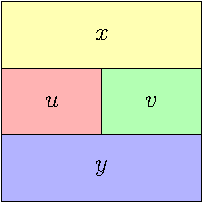
\includegraphics[height=29mm]{Resources/FlipInternalEdge-Example-2.pdf}}
	\qquad
	\subfigure[]{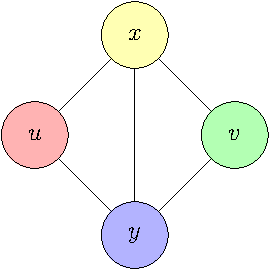
\includegraphics[height=29mm]{Resources/FlipInternalEdge-Example-3.pdf}}
	\quad
	\subfigure[]{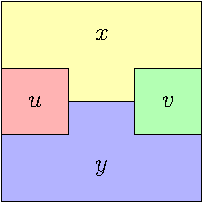
\includegraphics[height=29mm]{Resources/FlipInternalEdge-Example-4.pdf}}
	\caption{A cluster graph and a polygonal dual thereof, before (a, b) and after (c, d) flipping the internal edge $\{u,v\}$.}
	\label{fig:flip-internal-edge-example}
\end{figure}

An edge flip in a cluster graph translates to region adjacencies being flipped in its dual. Given a polygonal dual of some cluster graph, we apply an edge flip in two phases. First, we contract the respective region boundary into a single point, creating a degenerate contact representation in which 4 regions meet in a point. In the second phase, we create a new boundary in the opposite direction around that point the original boundary has been contracted into.

%Let us \todo{} using the example of \cref{fig:flip-internal-edge-example}.
%We now provide a detailed description using the example of \cref{fig:flip-internal-edge-example}.
%We start by computing the path $P_{uv} = (p_0, \dots, p_n)$ forming the boundary between the faces $u$ and $v$.

We contract a region boundary by repeatedly removing a peripheral edge of the boundary on alternating ends until the last edge of the boundary has been removed. To remove a peripheral edge of a boundary, let us consider the general case illustrated in \cref{fig:flip-internal-edge-contract}. We want to get rid of the edge $\{p_1,p_2\}$ on the red-green boundary. To do so, we  remove $p_2$ and its incident edges and add the new edges $\{p_3,p_1\}$ and $\{p_4,p_1\}$. This may introduce edge crossings though, as illustrated in \cref{subfig:flip-internal-edge-contract-crossing}. We may therefore need to introduce a bend to both new edges in the form of a subdivision vertex. We look for possible bend locations on the segment from $p_2$ to $p_3$ and $p_2$ to $p_4$, respectively, using binary search: We start at the far end, and cut the remaining distance to $p_2$ in half until we find a bend location that doesn't introduce edge crossings. As the distance from $p_2$ grows infinitesimally small, we are guaranteed to find a valid bend location.

\begin{figure}[H]
	\centering
	\subfigure[]{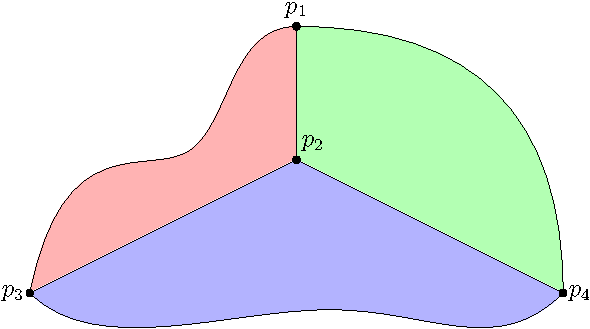
\includegraphics[width=40mm]{Resources/FlipInternalEdge-Contract-1.pdf}}
	\quad
	\subfigure[]{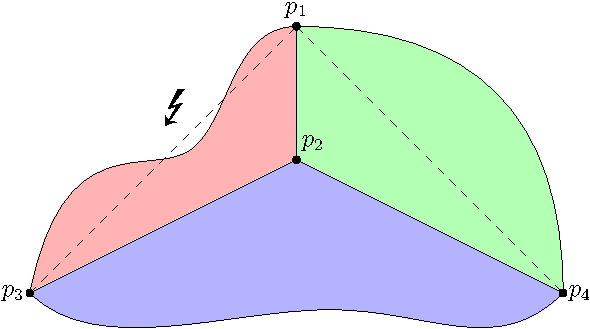
\includegraphics[width=40mm]{Resources/FlipInternalEdge-Contract-2.pdf}\label{subfig:flip-internal-edge-contract-crossing}}
	\quad
	\subfigure[]{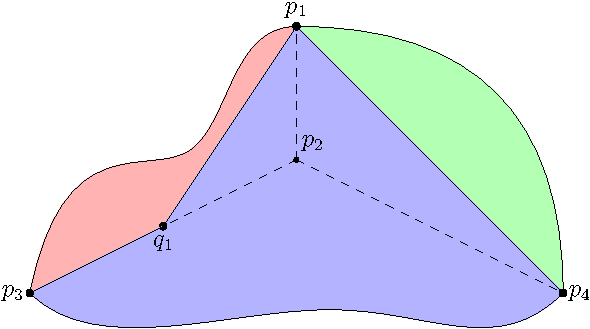
\includegraphics[width=40mm]{Resources/FlipInternalEdge-Contract-3.pdf}}
	\caption{A contact representation before (a) and after (c) removing the peripheral edge $\{p_1,p_2\}$ from the red-green boundary. (b) shows that we require a subdivision vertex $q_1$ on the red-blue boundary.}
	\label{fig:flip-internal-edge-contract}
\end{figure}

Once the boundary has been contracted into a single point, we need to resolve the degeneracy and create a boundary in the opposite direction as illustrated in \cref{fig:flip-internal-edge-expand}. If $\measuredangle_{p_1p_3p_4} < 180^\circ$, we search for a position in the face bounded by $p_1$, $p_3$, and $p_4$ at which we can place a new vertex $q_1$ and connect it to those three vertices without introducing edge crossings. We do this using another binary search on the segment from $p_3$ to the midpoint of $p_1$ and $p_4$. Once we found a valid position for $q_1$ and have added it to the graph along with the aforementioned edges, we remove the edges $\{p_3,p_1\}$ and $\{p_3,p_4\}$. We repeat the same for the face on the opposite side. Considering it is impossible for the angles to be more than half a turn on both sides, we have replaced at least one set of edges and have therefore successfully resolved the degeneracy and flipped the region adjacency.

\begin{figure}[H]
	\centering
	\subfigure[]{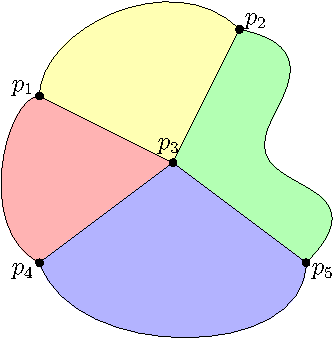
\includegraphics[width=30mm]{Resources/FlipInternalEdge-Expand-1.pdf}}
	\quad
	\subfigure[]{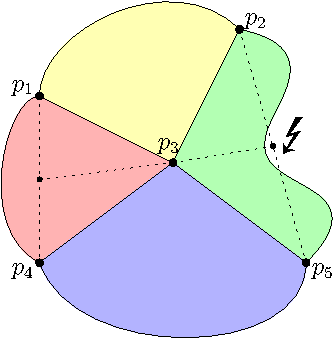
\includegraphics[width=30mm]{Resources/FlipInternalEdge-Expand-2.pdf}}
	\quad
	\subfigure[]{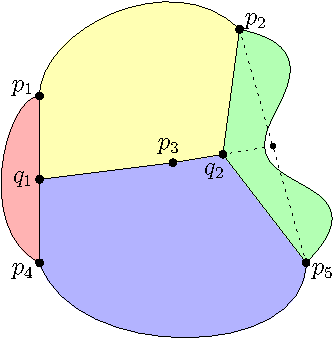
\includegraphics[width=30mm]{Resources/FlipInternalEdge-Expand-3.pdf}}
	\caption{A contact representation before (a) and after (c) creating a non-degenerate yellow-blue adjacency. (b) shows that $q_2$ cannot be the midpoint of $p_2$ and $p_5$ and needs to move further towards $p_3$.}
	\label{fig:flip-internal-edge-expand}
\end{figure}
